\documentclass[12pt,a4paper,titlepage]{article}

\usepackage[utf8]{inputenc}
% Set level to number headings on
% part = -1
% chapter = 0
% section = 1
% subsection = 2
% subsubsection = 3
% paragraph = 4
% subparagraph = 5
\setcounter{secnumdepth}{0}

% Table of contents level if added
\setcounter{tocdepth}{2}

% Header and footer specifications
%\usepackage{lastpage}
\usepackage{fancyhdr}
\pagestyle{fancy}

%url linebreaks
\usepackage{url}

% Add extra vertical whitespace for each new paragraph
%\setlength{\parskip}{5pt plus 1pt minus 1pt}

\headheight = 28pt
\lhead{Sensor data aggregation through CoAP}
%\texttt{Work in progress}}
%\rhead{\thepage\ of \pageref{LastPage}\\} %// Requires LastPage latex module
\rhead{} % Remove to enable Section name in the header
%\cfoot{}
%\rfoot{}

% Images
\usepackage{graphicx}

%%%%%%%%%%%%%%%%%%
% Custom new commands
%%%%%%%%%%%%%%%%%%

% From http://en.wikibooks.org/wiki/LaTeX/Title_Creation
% Used for the title page
\newcommand{\HRule}{\rule{\linewidth}{0.5mm}}

% Start of our document
\begin{document}

%Start page numbering from first page
%\thispagestyle{empty}
%\end{titlepage}
\setcounter{page}{2}

%Include the different parts in the lab report
% EXAMPLE: Sections and Paragraphs
% \section		- Level 1
% \subsection		- Level 2
% \subsubsection	- Level 3
% \paragraph		- Level 4
% \subparagraph		- Level 5 
% \section{<NAME_OF_SECTION>}

% EXAMPLE: Include graphics 
% \includegraphics[width=130mm,height=108mm]{intro4.png}

% EXAMPLE: Nested list
%\begin{enumerate}
%\item Nested list
%\begin{enumerate}
%\item
%\item
%\item
%\item
%\item
%\end{enumerate}
%\end{enumerate}


%%%%%%%%%%%%%%%%%%%%%%%%%%%%%%%%%%%%%%%%%
% Basic title page structure copied from 
% http://en.wikibooks.org/wiki/LaTeX/Title_Creation
%
% Christoffer Holmstedt on the 
% 17th of february 2012
%%%%%%%%%%%%%%%%%%%%%%%%%%%%%%%%%%%%%%%%%
\begin{titlepage}
\begin{center}

% Upper part of the page
% TODO ADD GRAPHIC
%\includegraphics[width=0.15\textwidth]{./logo}\\[1cm]    
\textsc{\LARGE Luleå University of Technology}\\[0.5cm]
\textsc{\Large Third year project}\\[0.5cm]

% Title
\HRule \\[0.4cm]
{\huge Sensor data aggregation through CoAP}\\[0.2cm]

\HRule \\[1.5cm]

% Author and supervisor
\begin{minipage}[t]{0.5\textwidth}
\begin{flushleft} \large
{\bfseries \emph Authors:}\\
Sophia \textsc{Bergendahl}\\
\emph{sopber-8@student.ltu.se}\\[0.2cm]
Edvin \textsc{Bruun}\\
\emph{edvbru-9@student.ltu.se}\\[0.2cm]
William \textsc{Gustafsson}\\
\emph{wilgus-9@student.ltu.se}\\[0.2cm]
Christoffer \textsc{Holmstedt}\\
\emph{cihhol-7@student.ltu.se}\\[0.2cm]
Marcus \textsc{Rådman}\\
\emph{marrdm-9@student.ltu.se}\\[0.2cm]
Kristoffer \textsc{Svensson}\\
\emph{kirsev-9@student.ltu.se}\\[0.2cm]
Ludwig \textsc{Thurfjell}\\
\emph{ludthu-7@student.ltu.se}\\
\end{flushleft}
\end{minipage}
\begin{minipage}[t]{0.45\textwidth}
\begin{flushright} \large
{\bfseries \emph Supervisors:} \\
Ulf \textsc{Bodin}\\
\emph{ulf.bodin@ltu.se}\\[0.2cm]
Jens \textsc{Eliasson}\\
\emph{jens.eliasson@ltu.se}\\[0.2cm]
Rumen \textsc{Kyusakov}\\
\emph{rumen.kyusakov@ltu.se}\\[0.2cm]
\end{flushright}
\end{minipage}

\vfill

% Bottom of the page
{\large \today}

\end{center}

\end{titlepage}

% EXAMPLE: Sections and Paragraphs
% \section		- Level 1
% \subsection		- Level 2
% \subsubsection	- Level 3
% \paragraph		- Level 4
% \subparagraph		- Level 5 
% \section{<NAME_OF_SECTION>}

% EXAMPLE: Include graphics 
% \includegraphics[width=130mm,height=108mm]{intro4.png}

% EXAMPLE: Nested list
%\begin{enumerate}
%\item Nested list
%\begin{enumerate}
%\item
%\item
%\item
%\item
%\item
%\end{enumerate}
%\end{enumerate}
\pagenumbering{arabic}
\setcounter{page}{2}
\tableofcontents
\newpage
\section{Project Description}
\subsection{Background}
Luleå University of Technology conducts research on lowpower wireless microprocessors called "Mulle". 
These microprocessors can be used for various things depending on which type of sensors you connect to it, everything from measuring temperature or vibrations in a car to analyzing the quality of the road that you drive on.

Every year northern parts of Sweden are used for testing cars during winter conditions.
First you decide what you want to test in the car, then you do this by placing local sensors within the car.
When enough data is collected you return back home.
At the testing facility the data is now available for analysis.
Depending on the results from the previous runs you might want to test some parts in more detail so you re-configure all sensors and go out for another test run.

This process is time consuming when you need to return to testing facility to be able to analyze and re-configure all sensors.
In todays society most computers are connected to internet and/or other private networks, most of these computers have the ability to be remotely configured and maintained.
The goal with the project is to be able to analyze data from sensors in realtime and re-configure them on the fly while testing is in progress.
\subsection{Project Targets}
\begin{enumerate}
\item Be able to send live sensor data from multiple "Mulles" to an online logging server/service.
\item Be able to read sensor data on the web with both a PC (web browser) and through an Android mobile device.
\item Be able to re-configure the sensors through a web interface and through an Android mobile device.
\end{enumerate}

\subsection{Technical limitations}
The technical limitations for this project was mainly to restrict how flexible the finished solution was.
The Mulles can be used together with any kind of sensors.
In this project the main goal was to get it operational in a car and measure temperature and some other variables.


%TODO: Vad har explicit uteslutits från arbetet?

% EXAMPLE: Sections and Paragraphs
% \section		- Level 1
% \subsection		- Level 2
% \subsubsection	- Level 3
% \paragraph		- Level 4
% \subparagraph		- Level 5 
% \section{<NAME_OF_SECTION>}

% EXAMPLE: Include graphics 
% \includegraphics[width=130mm,height=108mm]{intro4.png}

% EXAMPLE: Nested list
%\begin{enumerate}
%\item Nested list
%\begin{enumerate}
%\item
%\item
%\item
%\item
%\item
%\end{enumerate}
%\end{enumerate}

\section{Execution of the project}
\subsection{Scrum and how it has been used}
It was decided back in November that the entire project would be divded into three sprints.
The exact dates were to be decided in the beginning of each sprint.
In cooperation with the client the scope of the project and the scope of the first sprint was decided upon in November.
During the first project meeting the first sprint goal was divided into eight sprint stories.
It soon became clear that those eight stories were way to big, at the end of the sprint none of the stories had been finished.

Lesson learnt, the second sprint was divided into smaller stories which gave immidiate result when the first 69 sprint story points finished during the second sprint.

To decide upon scope for each sprint story, for the second and third sprint, "planning poker" \cite[p.~42]{kniberg07} was used.
For every sprint story each project member wrote down an estimate on the scope for each story.
With planning poker it became clear that each project member had a different vision for each story.
A short discussion after each estimate made it more clear on how big the scope was, an agreement was usually made within a few minutes.

\subsection{One project, three sprint goals}
As mentioned earlier the project was divided into three sprints.
This meant that three different sprint goals had to be divided into smaller sprint stories which in turn had to be assigned to a project member.
Due to all project members being new to most of the tasks at hand the first team division was made with focus on components \cite[p.~106]{kniberg07}.
The goal with this was that each smaller team within the project could work together and dive deep into their specific part such as the Mulle, the server parts or the android code.
Later on, a split into cross-component teams \cite[p.~107]{kniberg07} was aimed for but due to some persistent bottlenecks in some components this was never done.

For all sprints the sprint planning meeting was used to categorize each sprint story into the different components (Mulle, Server, Android).
It was then up to each component based team to split their stories between themselves.
This ended being a very flexible solution and in some cases, too flexible. 
This lead to teams not using the Scrumboard online at Scrumdo.com and wander off from the sprint story they were supposed to work on.
For the last sprint everyone got at least one sprint story assigned to themselves directly during the sprint planning meeting.
This was made to put more focus on using the Scrumboard at Scrumdo.com.

A move to cross-component teams was never made, instead an attempt to increase development speed for the Mulle and the Android components were made by moving one team member from the server team to the Mulle team and another to the Android team.
The server component at this time was ahead of the other components.
A week later it became clear that the additional team member for the Mulle team was not needed, because the problem was still a bottleneck that only one or two team members could work on at a single point in time, a move back to the server team was made.

\subsection{Individual time monitoring and speed}
\subsubsection{Sophia Bergendahl}

\paragraph{Generally about time estimation}
Time estimation is something that I have found difficult to do, and it is something that shows in the three stories below. In the stories I have tried to find reasons to why the time 
estimation was inaccurate. Generally I believe the estimation was inaccurate because of inexperience, when having done something once it is easier to estimate time, but if it is the first time it 
is more difficult. If I had known more about the stories before doing them and if I in the past had reflected more about how fast or slow I work, I believe my time estimation would have been 
better.


\paragraph{Three stories}
\begin{enumerate}
\item{"Create a PHP-web page that presents information stored in the database."}

I had no experiences in creating a web page so I estimated that it would take me about eight hours, first to learn the basics about html, php and css, and then to implement it. It took me
about 12 hours, I believe it took longer because of the problems I had with retrieving data from the database and that I decided to split the php file containing the finished web page
into three parts header, main and footer to make it easier to add to the page. 

\item {"Add a button to the web page that can call Mulle-services on the server"}

I had some experience with php so I estimated that it would take me about four hours, which was about what it took for me to create a php form, understand how it works and connect it to a
python script that can call Mulle-services. I believe that since I had worked with php before it made it easier to estimate time. Furthermore if the  button I made had not been turn on/off
lamp, whose services is not implemented on the server, it would have taken me longer to finish because the python script I created need information about the service to call to work
fully. 

\item {"Create a database that keeps track of connected/active devices."}

I estimated that it would take me about eight hours, since I had no experience with databases, more than retrieving information from one. It took me about six hours, the reason to why it was
created quicker than expected was because I had few problems and I did not have the possibility to test it with a Mulle due to its communication problems.
 
\end{enumerate}	
\subsubsection{Edvin Bruun}
Throughout the project I, as well as my fellow group members, have been gradually learning to work with the Scrum project-model.
This work-model includes a tactic for distributing work called ''stories''. These stories are given a time estimate and an actual time when they are done, 
and following this I will explain three stories that I've encountered in this project. 
For convenience I've chosen one story from each iteration to roughly show how the work-model was more and more used. As a quick reminder, my stories have revolved around getting the Mulle-communication to work.

To start things off, I chose the first story that I had, which was titled ''CoAP communication over bluetooth from Mulle to server''.
This story was estimated to take the entire first sprint which was roughly eight weeks long. In this story there was a pretty hefty start-up time included, 
as most of us were clueless as to how much time we would spend on learning the new technologies in each of our assignment-fields(Mulle, Server, Android).
When the eight weeks were up, the progress on the story was horrible to say the least. During our first sprint we struggled with issues that were very much 
out of the scope of what we should have been doing. The reason for this was mainly because we needed to get these things working before we could start progressing on the actual story.
However when the time was up we agreed that we'd have to take a different route to achieve the communication so the actual time for this story was pretty accurate.

Moving on to the next story, this story took place in the second iteration and revolved around sending UDP packets from the Mulle to the server.
The point of this story was to check if we could achieve the simplest of communication(with our new approach) and then build from there. This story was scheduled to run over 
a week  which also was our estimate. The actual time for this story was however a few days over the estimate. The reason for this was that at this point we were working on multiple stories as
well as some issues with our testing methods. Looking back on the things that caused the delay I don't see how we could have avoided them.

The third story to be explained in this documentation is a story that was very small and which took place in the third iteration.
The task in the story was to get the Mulle to run a certain function every time it received a UDP package. This was estimated at roughly ten hours, 
were as the actual time it took was closer to five. The reason for the shorter time than anticipated was that I had gained knowledge how to do this 
indirectly through another story which I'd worked on earlier.

\subsubsection{William Gustafsson}
One of the main things about android that I've learnt is that it takes time, there's alot of documention that needs to be read and most of the guides already assumes that you know everything about android, except the part that you're looking up.

\noindent In the first iteration I was working with setting up everything needed to program Android. This means getting eclipse and it's plugins, android adb and all the other software working. 
Then I threw myself in and started working with the Bluetooth part of the application, my thoughts on this was that it wouldn't be so hard to get working. 
Reality then showed me otherwise and it both took alot more time than anticipated and didn't turn out as I had wished,
this mostly since I realised Android wasn't capable of doing the features wanted without changing things in the android operating system. This howeber gave me a grip of how I was supposed to
do when programming android. So the second iteration I used some time doing the basic android stuff like the manifest and getting the xml and logic of the application to work together. 
This would have taken alot more time without the help of Karl Öhman, fourth year student at Luleå University of Technology.             
\smallskip

\noindent Another story of the second iteration that actually was finished within the expected time was to design how the GUI would look, I did a couple of designs and asked around for which seemed like the best option, and
the result of that choice has been alot of the work done since. So since the basic Android things were working and the GUI and logic of the lists in 
the application were pretty close tied in Android programming I took the responsibility for those stories. They've been pretty time consuming since there has been alot of going back and forth in them since the 
basic components weren't capable of producing the result sought.

And now lastly, about my experience with this. Firstly I thought scrum was not really necessary and only a waste of time. But using it for a while I realised that knowing your speed and being able to break down problems in the way scrum was meant to be used, are really useful tools that can be used to speed up the project alot. About the android, well some of the things I've learnt is that before you can start coding the project there are alot of small things that must be done, of which most are kind of hard to find unless you know what you're searching for.

\subsubsection{Christoffer Holmstedt}
What I've learnt during this project is that there is no way to estimate a reasonable time without knowing something about the topic of concern beforehand.
I've had several stories assigned to me in the topic of linux installation and configuration e.g. installing a webserver and a mysql database.
Both the webserver and database I've installed several times before and knew exactly which steps I was supposed to do to get it up and running as soon as possible.
Of course this made it really easy to estimate an expected time for these stories, or at least most of them.
One story was about installing Ubuntu.
Even though I have installed Ubuntu several times before I didn't anticipate that an entire installation could be so slow, I had simply missed to take into account that we were running our server on a very old machine.
The time estimate for this story was of by 100\%.

The other stories that didn't go so well was mainly about python programming and working with the coapy server implementation. 
It took generally more time than I expected to get started.
In the future I will increase the expected time before I get going e.g. the time to read about a new software I will work with and the time to try out the current functionality.
Though I will keep my estimate for the actual coding parts.

In the future when it's up to me to do another estimate concerning a topic I've never worked with I hope I have a few colleagues with knowledge in that area to help me out with my first estimate.
As long as I guess an estimate instead of chosing "I don't know" I will improve and eventually I will know my "speed".

\subsubsection{Marcus Rådman}
My main task during the first sprint was to understand how the library jCoAP worked, eventually when I understood jCoAP somewhat I tried together with William to make it work together with Bluetooth.
Not knowing how anything worked made it almost impossible to make good estimations of how long tasks would take to complete.
Eventually when we scraped our attempts to send CoAP over Bluetooth in the beginning of sprint two, there were no longer any major problems to send an empty CoAP packet.
I expected it to take six hours in order to be able to send a packet with customised payload, this estimation included a large margin in case of unexpected problems. After nine hours I got it to work.
With that behind me I tackled the issue of being able to receive messages as well. To my surprise, this worked almost "out of the box" and only took one hour to implement and test instead of the expected two.
After that I dealt mostly with minor issues that never got written down at the Scrum-board.

Working by Scrum has been quite difficult.
There has been many smaller fixes, things to learn how it works and other minor issues that have been difficult to write down as a Scrum-point.
The biggest problem has actually been the fact I didn't know how Android works, this was something I had to learn.

Personally, if I got the chance to redo the project I would first insist on a better and more thorough planing of the program structure of the Android application.
Another thing I would like is to be better at dividing the big tasks into smaller tasks, something like a clear program structure would have made it a lot easier to do.
The problems of working with something you have never worked with before can not be avoided. Well structured work can however limit the effects of this.


\subsubsection{Kristoffer Svensson}
\paragraph{Assignments}
\begin{enumerate}
\item{"Restructure the loading of new services for the python server"}

I had some previous experience with python on top of already been dealing with the actual server implemention we decided to use prior to dealing with this issue so I was pretty certain I would be able to complete it in about 3 hours.
Without any major issues I managed to complete it in roughly 3 hours and 30 minutes. The question at that point was rather if the solution was adequate, which after some consultation it was deemed to be.

\item {"Figure out how service discovery works in CoAP"}

The estimated time for this was set between 8 and 10 hours. The reason being that it was new ground for me but still didn't feel like it was that big of
an issue. It turned out to be a relatively small fix after 6 hours of work. The issue of whether the solution was good enough or not for the end-purposes was brought up again but it was decided that it was good enough for the time being.
With that said, I doubt that the estimated 8-10 hours would have been sufficient if a end-purpose qualifying solution was to be made. 

\item {"Implement EXIficient"}

Originally the time for this assignment was set to 20 hours, when the assignment was still "Implement EXI parser". In that situation we assumed that there was more work to be done making the parser from the ground up.

When EXIficient was discovered we found out that it had a ready-made demo that almost suited our needs. It turned out that the actual time needed to get something that would do the job for us would be around 10 hours modifying that demo.

\item {"Individual documention"}

I assumed about 2-4 hours for the actual writing with an added hour or two for the research needed to know what was to be included in the report. In the end, this all came down to about 4-5 hours which is well within the expected range.

\end{enumerate}

\paragraph{General thoughts concerning time estimation}

I feel as if my personal time estimations, contrary to what I expected, have been quite accurate. I reckon the reason for this being that I had the fortune of having some kind of knowledge concerning the assignments prior to doing them. Without any idea on the scope or size of the assignments I think that the estimations wouldn't have been this accurate.

The estimations themselves have been useful tools for knowing when to ask for help or guidance. When you're approaching a time limit and you know that you're kind of stuck that's a really good indicator that help is needed. I think it's been quite a useful tool, at least for me personally.

\subsubsection{Ludwig Thurfjell}
The project group was divided into three groups, one for C-coding on the Mulle, one for Android phone
and one to set up the server. I was part of the two-man group for the Mulle. We worked with the Scrum model 
for the project, thus there were stories and iterations. 

We had three iterations in total in this project, with sprint planning and what we would like to demo at the 
end of each period. I will show three different stories I've participated in, and so one clearly can see
how the project has matured from day one to the last.

Ideally what I have experianced in the course, is that you need to really break down problems into very small
parts, thus creating many smaller stories which can be significantly easier to estimate the time of. The joy of completing
something is also more rewarding, even though there are small steps to the way of the big picture. It's very demoralizing to 
have a single giant problem to beat.

In the first iteration, we had a story called ''CoAP communication over bluetooth from Mulle to server'', with a huge score
in the estimation part of the sprint planning. Needless to say this story was enormous and involved so much work which at the start
was very hard to imagine. Thus the time estimation of this story was very unstable. Without any knowledge of the CoAP protocol or about the Mulle, this story could take a week or months.

The project changed a bit in term of content and I will jump to describe two stories from the third and last iteration.
One of my stories was ''Run appropriate functions from whatever server calls for''. Since I had read a whole lot about CoAP and 
the LWIP stack, I made a handler quite fast, although it wasn't possible to try it on the Mulle and develop it further since
we couldn't at any stage of the project get simple communication working. Thus the code was scrapped, but the time estimation was somewhat
correct in regards that it would probably have taken lots of time to debug and implement it. 
This story could easily have been broken down to smaller parts as well.

Last story I will describe is ''Internet to Mulle from computer running Bluesoleil''. This one was rated with a low score, which is 
very reasonable. It took less time than expected to complete this story since the installation was straightforward, and the conclusion
that it doesn't work at all was quickly made.

\subsection{Reflection about Scrum usage during this project}
A lot has been learnt during this project and to keep it short the following lessons learnt and improvements that can be made are a chosen few.

At the end of all projects when the deadline is closing in the pace of the development often increases.
A downfall of this is that when the speed increases the quality of the code often decreases.
Scrum is a solution to this problem with the main goal of keeping a steady development pace and always keeping the quality of the code as good as possible above some minimum criteria.
With too long sprints, projects will still end up with a big deadline, this is what happened in this project.
In total the project lasted about 17 weeks including the winter holidays.
Instead of three sprints where each lasted about five weeks a project split into smaller sprint would have been better.
If time travel was possible this project would have had two smaller sprints in the beginning each would have lasted for two weeks.
The first sprint with goal of configuring all required software for everyone such as setting up git, the different IDEs, gcc and other required software/tools.
The second sprint with the goal of understanding what was available at the time and get all basic functionality working.
If the project had found any big bottlenecks at the end of the second sprint that would be the point in time to halt the project and really rethink what to focus on.
The remaining weeks should have been divided into three evenly sized sprints.

Another big improvement could have been made in the relation between Scrum team and product owner.
From the beginning it was unclear who was the product owner out of three supervisors/clients, this should have been defined to one single person as early as possible before continuing with any other work.
The absence of the product owner before and during our sprint planning meetings resulted in a lot of confusion when it was up to the team to decide an estimate for each sprint story.
The lesson learnt from this is that without a product owner the scrum team will fumble in blindness forever or as Kniberg writes \cite[p.~25]{kniberg07} {\em "...each story contains three variables that are highly dependent on each other"}.
There is no way the team can choose a good estimate when there is no product owner that has already chosen an importance and scope for each sprint story to start with and is available to change that during the course of a sprint planning meeting.
This also lead to the project growing in scope without any clear bounds.

The last and perhaps the most important improvement that will be mentioned is the importance of having a team member taking the role as Scrum master.
Without the Scrum master during the first sprint everyone was on their own.
For the second and third sprint the Scrum master role was appointed to one team member.
This improved the communication within the Scrum team a lot and also made it possible for individual team members to have someone to go to in case of general questions and/or other problems.

%
% Andra kommentarer som kan vara värda att ta med om Scrum och hur det 
% har använts i detta projekt om det får plats. Texterna är redan lite för långa.
%
%TODO: Tydligare sprint mål för varje sprint från kravställare. En mening som beskriver syftet med respektive sprint.
%TODO: Tydligare demo av varje punkt
%TODO: Vi skulle ha satt ner foten på hur många delar vi skulle jobba med samtidigt. Startat med Mulle och Server enbart...sedan android i mån av tid för att få mer fokus i projektet, vi var trots allt bara sju personer.
%TODO: Ingen "experthjälp" med android tillgänglig. I detta läge gör det stor skillnad om man är två, tre eller fyra. Varje programmerare ökar hastigheten med mer än bara sin tid hen kan lägga till eftersom felsökning oftast går betydligt snabbare för fler personer än enbart två. Många fel beror också på utvecklingsmiljön, om man är fler med samma miljlö så är det större chans att någon har stött på problemet tidigare och har en lösning.
%TODO: Reflektion över flytten av individuella team members server till mulle och android. Väldigt "dyrt" i uppstartskostnad.

% EXAMPLE: Sections and Paragraphs
% \section		- Level 1
% \subsection		- Level 2
% \subsubsection	- Level 3
% \paragraph		- Level 4
% \subparagraph		- Level 5 
% \section{<NAME_OF_SECTION>}

% EXAMPLE: Include graphics 
% \includegraphics[width=130mm,height=108mm]{intro4.png}

% EXAMPLE: Nested list
%\begin{enumerate}
%\item Nested list
%\begin{enumerate}
%\item
%\item
%\item
%\item
%\item
%\end{enumerate}
%\end{enumerate}

\section{Results}
\subsection{Deliverables}
Mainly due to being unable to setup communication from the Mulle to the server, project target number one listed in the beginning of this document is not met.
What is delivered from the project concerning this is available in Appendix A where a guide on how to get started where this project ends is available.

Project target number two is not met.
What is delivered from the project is a basic webapplication with a simple database structure as the back-end where future real sensor data can be stored.

Project target number three is not met.
Basic functionality on how to use EXI as encoding for sensor data is available for the Mulle and the Android application but hasn't been tested.
No work on EXI has been made for the server though there exist a simple webpage to turn a value on or off.

\subsection{Testing}
During this project testing has been made by each project member.
The scope of the testing for each story has been up to each project member to decide upon.
Right before each sprint demo a project meeting was scheduled were each one showed what was completed and what was not.
Depending on what was ready at that point in time the entire Scrum team decided what was going to be presented at the demo and a test was made to confirm that it was possible to show the parts that were decided upon.
No further testing was made during this project.
\subsection{Lessons learnt}
Communication is always troublesome, it's usually easy to get a system to transmit data and another to do the same.
The hard part is when you want different system to actually communicate with each other.
This boils down to the lesson learnt that the project should have focused more on specific components instead of spreading out on all three components (Mulle, Android and the server) from the beginning.
The goal should have been to get the Mulle communicate with either the server or the android device to begin with.
When that was operational new systems could have been added to the mix.

Testing is always hard to do, it might be easy to test specific test cases but is very hard to test all possible usages.
To make sure that your codebase doesn't become useless in the long run you need somekind of automated testing to make sure that all previous bugs found are tested automatically with all new improvements and add-ons.
It might be time consuming in the beginning of a project but it's priceless in the end.
An important part of testing is to test both individual components and interaction between different components.
If only testing is made to the interaction between different components a finished component cannot be tested until the other one is finished aswell, this creates bottlenecks for the entire project.

When is something done?
Do not let this question be up to the individual programmer, it puts the programmer in a difficult situation.
Either the programmer wants to create the perfect spot and keeps going forever or the programmer will take shortcuts that will comeback and haunt you later on.
It must be up to the team to decide when something is done or not.
This will make it a lot easier in the day to day work for everyone, if anybody is uncertain if it's completed or not, just look into what was decided earlier.
\subsection{Suggested improvements}
Without meeting any of our project targets it's hard to suggest improvements except the obvious one to complete what has been started. 
Instead of going straight at it and try to finish it all as soon as possible some thought process need to be put into the question, what really needs to be finished?

From this projects point of view the first thing to prioritze is to get some communication with the Mulle.
The Mulle in its current state has a lot of bugs which makes it hard to debug, there seems to be a lot of "random" bugs occuring when you lest expect them. 
The code that is finished "should work" but hasn't.

The second priority should be to rethink the servers purpose.
At the current state the python implementation is very simple and if the only thing you want to do is add new CoAP services which just return some simple results, then keep going with the current server implementation.
A new service is very easy to add.
What has been realized at the end of this project is that in the long run it might be better to create a new C server implementation instead.
The main reason for this is that when you want to implement custom communication protocols such as EXI a lot of code is available in C and with a server implementation in C it will be relatively easy to share code between the server and Mulle system.

As the third and last priority, work should be put into the Android system. With the Mulle up and running for testing purposes it should be easy to get going with the android application but without the Mulle the android application isn't worth anything.


% TODO: Fortsätt på Mullen
% TODO: Tänk efter om CoAPy är rätt väg att gå
% TODO: Skippa android tillsvidare om den inte är viktigare än servern.

%
% Scrum och relatera till våra referenser \cite{kniberg07}
% \cite[p.~107]{kniberg07}
%

% EXAMPLE: Sections and Paragraphs
% \section		- Level 1
% \subsection		- Level 2
% \subsubsection	- Level 3
% \paragraph		- Level 4
% \subparagraph		- Level 5 
% \section{<NAME_OF_SECTION>}

% EXAMPLE: Include graphics 
% \includegraphics[width=130mm,height=108mm]{intro4.png}

% EXAMPLE: Nested list
%\begin{enumerate}
%\item Nested list
%\begin{enumerate}
%\item
%\item
%\item
%\item
%\item
%\end{enumerate}
%\end{enumerate}

\section{Conclusions}
This project started out to be of reasonable size for our project group but ended up way too big mainly due to some persistent bottlenecks in some components.
This lead to no component (Mulle, CoAP server and Android application) being fully functional in the end.
This is exactly what Scrum tries to prevent, as discussed earlier in this report a better solution to improve quality would have been to do a few more, but smaller sprints.

Concerning usability and future improvements there is a lot more work that needs to be done.
The current state of the the software is that all components are lacking small parts in different areas, this makes it unusable in it's current state.
Future improvements should start with taking a step back and really rethink what the goal is and start working with one component at a time.
Highest priority should be to get the Mulle operational and able to communicate with it's surroundings.
Without sensors there is no data to analyze or to reconfigure "on the fly".

% EXAMPLE: Sections and Paragraphs
% \section		- Level 1
% \subsection		- Level 2
% \subsubsection	- Level 3
% \paragraph		- Level 4
% \subparagraph		- Level 5 
% \section{<NAME_OF_SECTION>}

% EXAMPLE: Include graphics 
% \includegraphics[width=130mm,height=108mm]{intro4.png}

% EXAMPLE: Nested list
%\begin{enumerate}
%\item Nested list
%\begin{enumerate}
%\item
%\item
%\item
%\item
%\item
%\end{enumerate}
%\end{enumerate}

\begin{thebibliography}{9}

\bibitem{kniberg07}
    Henrik Kniberg,
    \emph{Scrum and XP from the Trenches}.
    C4Media Inc, Publisher of InfoQ.com,
    978-1-4303-2264-1,
    \texttt{http://infoq.com/minibooks/scrum-xp-from-the-trenches},
    2007.

\end{thebibliography}

% EXAMPLE: Sections and Paragraphs
% \section		- Level 1
% \subsection		- Level 2
% \subsubsection	- Level 3
% \paragraph		- Level 4
% \subparagraph		- Level 5 
% \section{<NAME_OF_SECTION>}

% EXAMPLE: Include graphics 
% \includegraphics[width=130mm,height=108mm]{intro4.png}

% EXAMPLE: Nested list
%\begin{enumerate}
%\item Nested list
%\begin{enumerate}
%\item
%\item
%\item
%\item
%\item
%\end{enumerate}
%\end{enumerate}
\section{Appendix A - How to build upon the codebase}
This appendix include information on how to build upon our codebase for the Mulle (C), server code (Python, PHP/HTML5 and C) and Android Mobile phone (Java).
\subsection{Mulle}
The Mulle communication via COAP is far from finished and therefore here is a guide how to get started followed by what should be further built. The instruction on how to get started are done in Ubuntu, the versions that were tested are 10.04 and 11.10. Windows or any other OS will not be covered in this guide.

The Mulle software required is all in the Software-PAN-NAP folder which contain necessary libraries and applications. It is assumed that you have acquired this because it's essential for any development.

\subsubsection{Getting started}
The first step you will take is to download the code from a repository on Github.com, if you don't know how to do this there are several guides how to do that on their site. Since there are several ways to do this here are the links to the repository:
\begin{itemize}
\item Download zip: \url{https://github.com/christofferholmstedt/vehicletesting/zipball/master}
\item Git: \url{git://github.com/christofferholmstedt/vehicletesting.git}
\item SSH: \url{git@github.com:christofferholmstedt/vehicletesting.git}
\end{itemize}
When you've done this note that you'll only need files from the ../vehicletesting/code/Mulle folder.
In this folder there are two subfolders named Coap and PAN-Router\_demo. 
These two folders are going to seperate locations in your Mulle software folder, 
since the Coap folder contains the code for the protocol and PAN-Router\_demo code for the application. 

The folder Coap should be copied into ../$<$Mulle Software folder$>$/Libary/misc/apps/ 
and the PAN-Router\_demo folder goes to  ../$<$Mulle Software folder$>$/Applications/. 
The PAN-Router\_demo folder is optional to use, if you want to use you're own Mulle program you need to include coap.h and run coap\_init() somewhere in your applications c-file. 
Since the coap-protocol isn't official you also need to put a "\#define LWIP\_COAP" and set it to 1 in proj\_arch.h(as well as turn off any other protocol that are used for communcation) 
and finally you need to add coap.c in the SOURCES.mk file. This is done by adding "\$(LIBDIR)/misc/apps/coap/coap.c" to the LWIP\_Apps field.

Now when you have the code set up you must install the gcc compiler, namely m32c-elf-gcc, for this type of hardware. Do the following steps in your terminal with sudo, alternatively make a script. Be prepared to redo this if you're doing it in a script. It's preferable to do this step by step because it has a higher rate of succeeding. 

Alternatively you can follow this guide(however, it's strongly advised not to): \url{http://www.eistec.se/docs/wiki/index.php?title=Mulle\_software\_with\_GCC}

Setup Development Host:
\begin{itemize}
\item apt-get install build-essential
\item apt-get install m4 autoconf libtool gawk bzip2 bison flex gettext texinfo zlib1g-dev 
\item apt-get install libmpc-dev libmpfr-dev
\end{itemize}

\noindent When this is done you need to download binutils and install it:
\begin{itemize}
\item wget \url{http://ftp.gnu.org/gnu/binutils/binutils-2.19.1.tar.bz2}
\item tar xjf binutils-2.19.1.tar.bz2
\item mkdir binutils-obj
\item cd binutils-obj
\item ../binutils-2.19.1/configure --target=m32c-elf
\item make
\item sudo make install
\item cd ..
\end{itemize}

\noindent In the next step you'll download gcc-4.3.3 and newlib 1.17 and install them:
\begin{itemize}
\item wget \url{ftp://ftp.nluug.nl/mirror/languages/gcc/releases/gcc-4.3.3/gcc-4.3.3.tar.bz2}
\item wget \url{ftp://ftp.nluug.nl/mirror/languages/gcc/releases/gcc-4.3.3/gcc-core-4.3.3.tar.bz2}
\item wget \url{ftp://sources.redhat.com/pub/newlib/newlib-1.17.0.tar.gz}
\item tar xjf gcc-4.3.3.tar.bz2
\item tar xjf gcc-core-4.3.3.tar.bz2
\item tar xzf newlib-1.17.0.tar.gz
\item cd gcc-4.3.3
\item ln -s ../newlib-1.17.0/newlib
\item ln -s ../newlib-1.17.0/libgloss
\item cd ..
\item mkdir gcc-obj
\item cd gcc-obj
\item ../gcc-4.3.3/configure --target=m32c-elf --with-newlib --enable-languages="c"
\item make
\item sudo make install
\item cd ..
\end{itemize}
When you've done all these steps you should try typing this into your terminal: "m32c-elf-gcc --version" and check that it says "m32c-elf-gcc (GCC) 4.3.3" just to be sure.

Now you're good to go, a final note on how get get set up is how to push your code onto the Mulle. Pushing your programs is done in a few steps, first you need to orient your way to the folder containing the program you're pushing in the terminal, then do these steps:
\begin{itemize}
\item make clean
\item make all
\item make program
\item make debug
\end{itemize}
The “make clean” is only needed if you changed something in the system files and when running “make program” the Mulle must be set to “Program Mode”. If all your modified files are correct your code will be pushed to the Mulle, if you get a “Clock Validation Error” make sure the Mulle is set to “Program Mode” and try again. The “make debug” command starts mulle\_term, which is a terminal debugger for the Mulle, so when you put it back on “Run Mode” you'll see what it is doing(in the form of printouts).

\subsubsection{Further developement}

You will need some sort of device that can share internet through Bluetooth to the Mulle, whether it be a telephone or a personal computer with an USB-dongle. To test COAP protocol, you can download the Copper addon for Firefox. The coap\_init() function in coap.c initializes so that when you receive UDP packets on the Mulle the function coap\_input() is run.

First the coap\_input() function needs to be properly made, since it does nothing useful at this time. What needs to be done is that the function should put all the correct values into a coap struct and based on what values are in each field the function should decide where to send the infomation next for handing. 

A suggestion for handling the COAP payload is by working with EXIP. You create and decode exi files directly on the mulle. EXI-files which have the same structure as XML are interesting for this type of projects since it's light and you can easily write scripts with XML structure.

You can find out more about EXIP here: http://exip.sourceforge.net/ .
A final suggestion is to finish the debug\_coap\_print() function since it will be very helpful for debugging.

\subsection{Server}
\subsubsection{Coapy server}
\paragraph{Existing implementation}
The server is based on CoAPy, which is a python implementation of the CoAP protocol. The actual server implementation is a modification of the example server provided along with CoAPy.
Some minor changes were made to it allowing it to accept all forms of CoAP messages, provided they are taken care of properly. We also added a way for new services to be easily added 
and used. 

The procedure when adding new services is as follows:
\begin{enumerate}
\item Create a new .py file with the name corresponding to the actual service name (e.g. "TestService.py") in the "services" directory
\item The file should contain only the necessary imports (including CoAPy parts) along with a class name the same thing as the file ("TestService", in this case)
\item The class is to define a single function "process" in which the actual actions of the service are to be made
\end{enumerate}

Using an existing service, like "CounterService.py", is highly recommended for understanding how a service should be structured and laid out.

\paragraph{Further development}
The server itself should be set to add new services for operation. What needs more work is the incorporation of a few things:

\begin{enumerate}
\item An actual XML scheme for configuration of mulle nodes. This point is not particular to the server, however.
\item Implement ways for the server to make use of the EXIP application to translate the XML that's to be sent into EXI via the command line.
\item Make services corresponding to the functionality you would like to have for configuration and communication with mulles and android devices, respectively.
\end{enumerate}
\subsubsection{Webpages and database}
 
The webpages and database consists of Apache2 which is an web server, MySQL which is a database management system and PHP which is a language for producing dynamic webpages.
LAMP (Linux), WAMP (Windows) or MAMP (Mac) can be used to build a web server it is an web-platform that consists of Apache, MySQL and PHP.

\paragraph{Webpages}

The webpages are built up using mulleheader.php which contains the header and sidebar, a .php file containing page content and mullefooter.php which contains the footer.

We have built two webpages using this concept; One that shows information from the database and its .php file that holds page content is mulledatabase.php and one consists of 
a php form to turn on or off a lamp and its .php file that holds page content is mullebuttons.php. The mullebuttons.php also contains a call to a .py file called testsender.py
that with some work can run a service on the CoAP server.


How to create a new webpage:

1. 	Create a new .php file for page content

2. 	In the top of the .php file print:\\$<?$php include("mulleheader.php"); $?>$

3. 	Between \\$<$ section id ="main" $>$ and $<$/section $>$ write the page content

4. 	In the bottom of the .php file print\\$<?$php include("mullefooter.php"); $?>$

\paragraph{Database}

We created a MySQL database and named it mulle and to this database we added two tables one that keeps track of communication on server and one that keeps track of connected/active 
devices. Online you can find many guides on how to add to a LAMP, WAMP or MAPM MySQL database, but down below shows some commands good to know when creating a database.  


How to create a new database:

1. 	Open up your MySQL Console and login

2. 	mysql$>$ \texttt{SHOW\ DATABASES};

3. 	mysql$>$ \texttt{CREATE DATABASE the\_database\_name;}

4. 	mysql$>$ \texttt{USE the\_database\_name}

5. 	\texttt{CREATE TABLE name\_of\_table (name\_first\_column\_in\_table VARCHAR(20), name\_second\_column\_in\_table VARCHAR(20), name\_date\_and\_time\ DATETIME);}
	This creates a table with three columns.
	
6. 	\texttt{SHOW\ TABLES;}

7. 	\texttt{EXPLAIN name\_of\_table;}

\subsection{Android Mobile Phone application}

The primary goals for the android applications were to;
%communication goes via a server.
\begin{itemize}
 \item communicate using CoAP over an UDP connection
 \item encode the sent packets with EXI to reduce the size of packets
 \item have a graphical UI capable of controlling multiple devices.
\end{itemize}
% UNDERSÖK OM MER SKA IN HÄR

\subsubsection{The goal of the finished product}

The application starts off by showing the server menu. One will have to either add a server or use a saved one. 
Clicking on a server in the list will cause the application to validate that the server is alive and thereafter it will perform a CoAP discovery on the server. 
When receiving an answer to the discovery the application will start filling the device menu with devices and their services. The device menu can then be accessed to use the services available.
The services generally works as follows: The application gets a click on the chosen service, so it sends its message to the service owner, whereafter the services device either changes something or responds.
The service owner will then have to respond to the Android application with the updates made, this can be with a confirmation or a whole new CoAP message. This makes the application respond by updating the GUI with the new values.\smallskip

The pre-built services are generalized to: 
\begin{itemize}
\item IsOn, provides an item with a checkbox that is checked if a service is on (for example a lamp). Clicking on this should provide a change on the selected device.
\item GetValue, provides an item which shows the last value provided. Clicking on the item should provide an update.
\item SendValue, provides an item which have a view of the current value and a textbox where one can send a payload to the device.
\end{itemize}

Another feature of the finshed product would be the options menu where the application will allow things like turning EXI encoding on or off. 

\subsubsection{What exists today}

Today there exists a communication part which allows one to send and recieve CoAP messages. This part uses a library made out of \texttt{jCoAP revision 202b8f8eb7b4, http://code.google.com/p/jcoap/}%s.unger.mobil@gmail.com committer ,	chr.lerche@gmail.com	owner,	nic@nclm.de	owner 
to get the CoAP features. The reason for making this a library is to make a Java project compile in the Android project without complications. The jCoAP project is not yet finished but the features requested for this application is present. The EXI converter is currently not available but is planned to use exificient, 
which can be found at \url{http://exificient.sourceforge.net/}.

The GUI is another important part of the application. It is built to be able to controll multiple servers and devices. 
To make this possible the application has 3 tabs:	%the default thought was to have a checkbox in the server menu to allow one to decide whether a server is being currently used, this idea has however been dropped due to lack of time.
\begin{itemize}
 \item Device tab
 \item Server tab
 \item Options tab
\end{itemize}

The Options tab does currently not contain anything but should simply allow a user to change things about how the application should work and what and how things should be displayed. 

\begin{center}
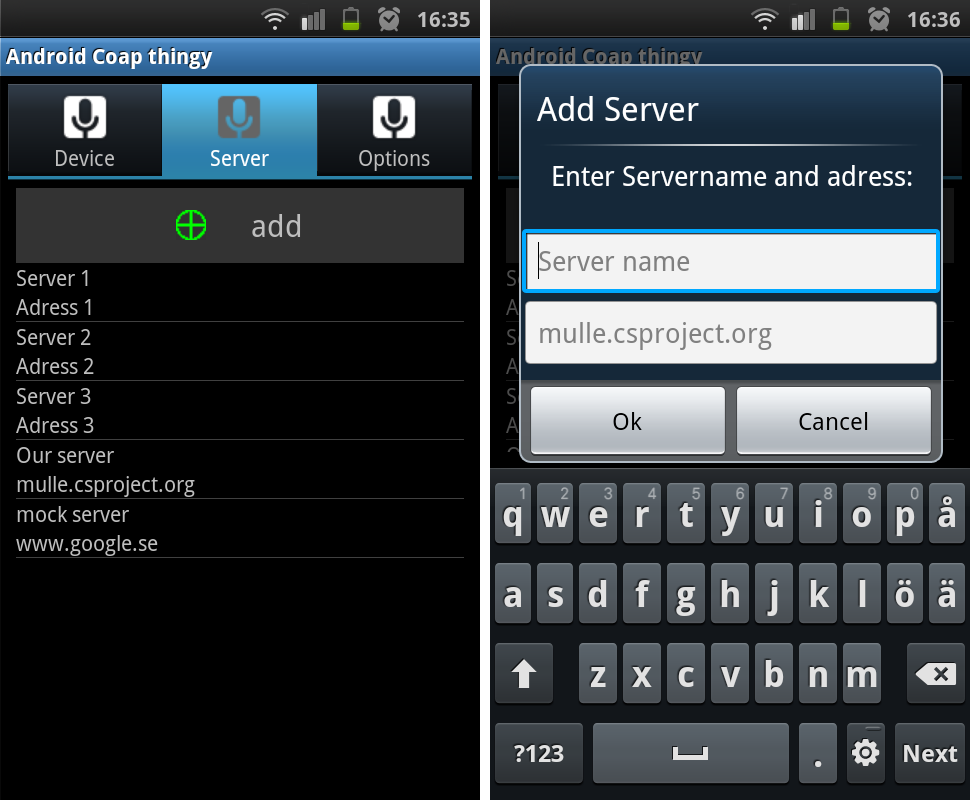
\includegraphics[scale=0.25]{android-server.png}%\caption{The Server tab of the Android application}
\end{center}
The Server tab shows all the active servers. You can click on the add button in the server menu and a window appears where you write in the name and adress appear. The servers then appears in a listview where it's easy to keep track of them. In the future this can be complemented with a network discovery of nodes, however, my personal opinion is that it should be possible to manually add an server.

\begin{center}
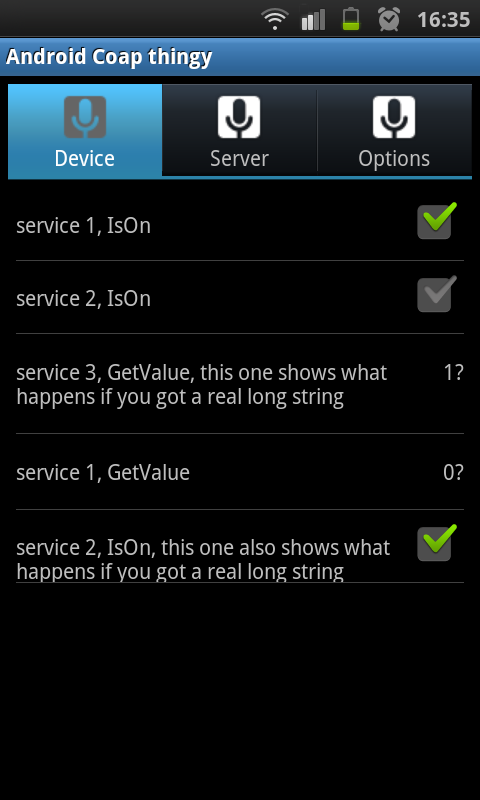
\includegraphics[scale=0.25]{android-device.png}%\caption{The device tab of the Android application}
\end{center}
The Device tab is the latest addition in the GUI and contains the actual services that are available. It contains a custom ArrayAdapter that have been tweaked to be able to display children of the interface rowdata.
In it's current state it is possible to add items to this list in the code by calling the NewItem() function with proper parameters. If the prebuild service types would not suffice it's relatively easy to add new ones.
Simply extend the rowdata() interface and create the desired xml for the item, do not however forget to add a typenumber for the NewItem() function to be able to create it. 
This also allows the children to define for their own what should happen if clicked, updated and so on.


\end{document}
